\subsubsection{Modification}

The modify flow are similar as \textit{STRING} type, remove the key which don't needed and add the count if the byte is the same. So follow the example in figure \ref{fig:algorithm:integer:insertion:example_1} and modify 167904506 (10-2-4-250) to 2 (0-0-0-2), the table will look like figure \ref{fig:algorithm:integer:modification:example_1} and time complexity is $O(b)$.

\begin{figure}[h]
\centering
%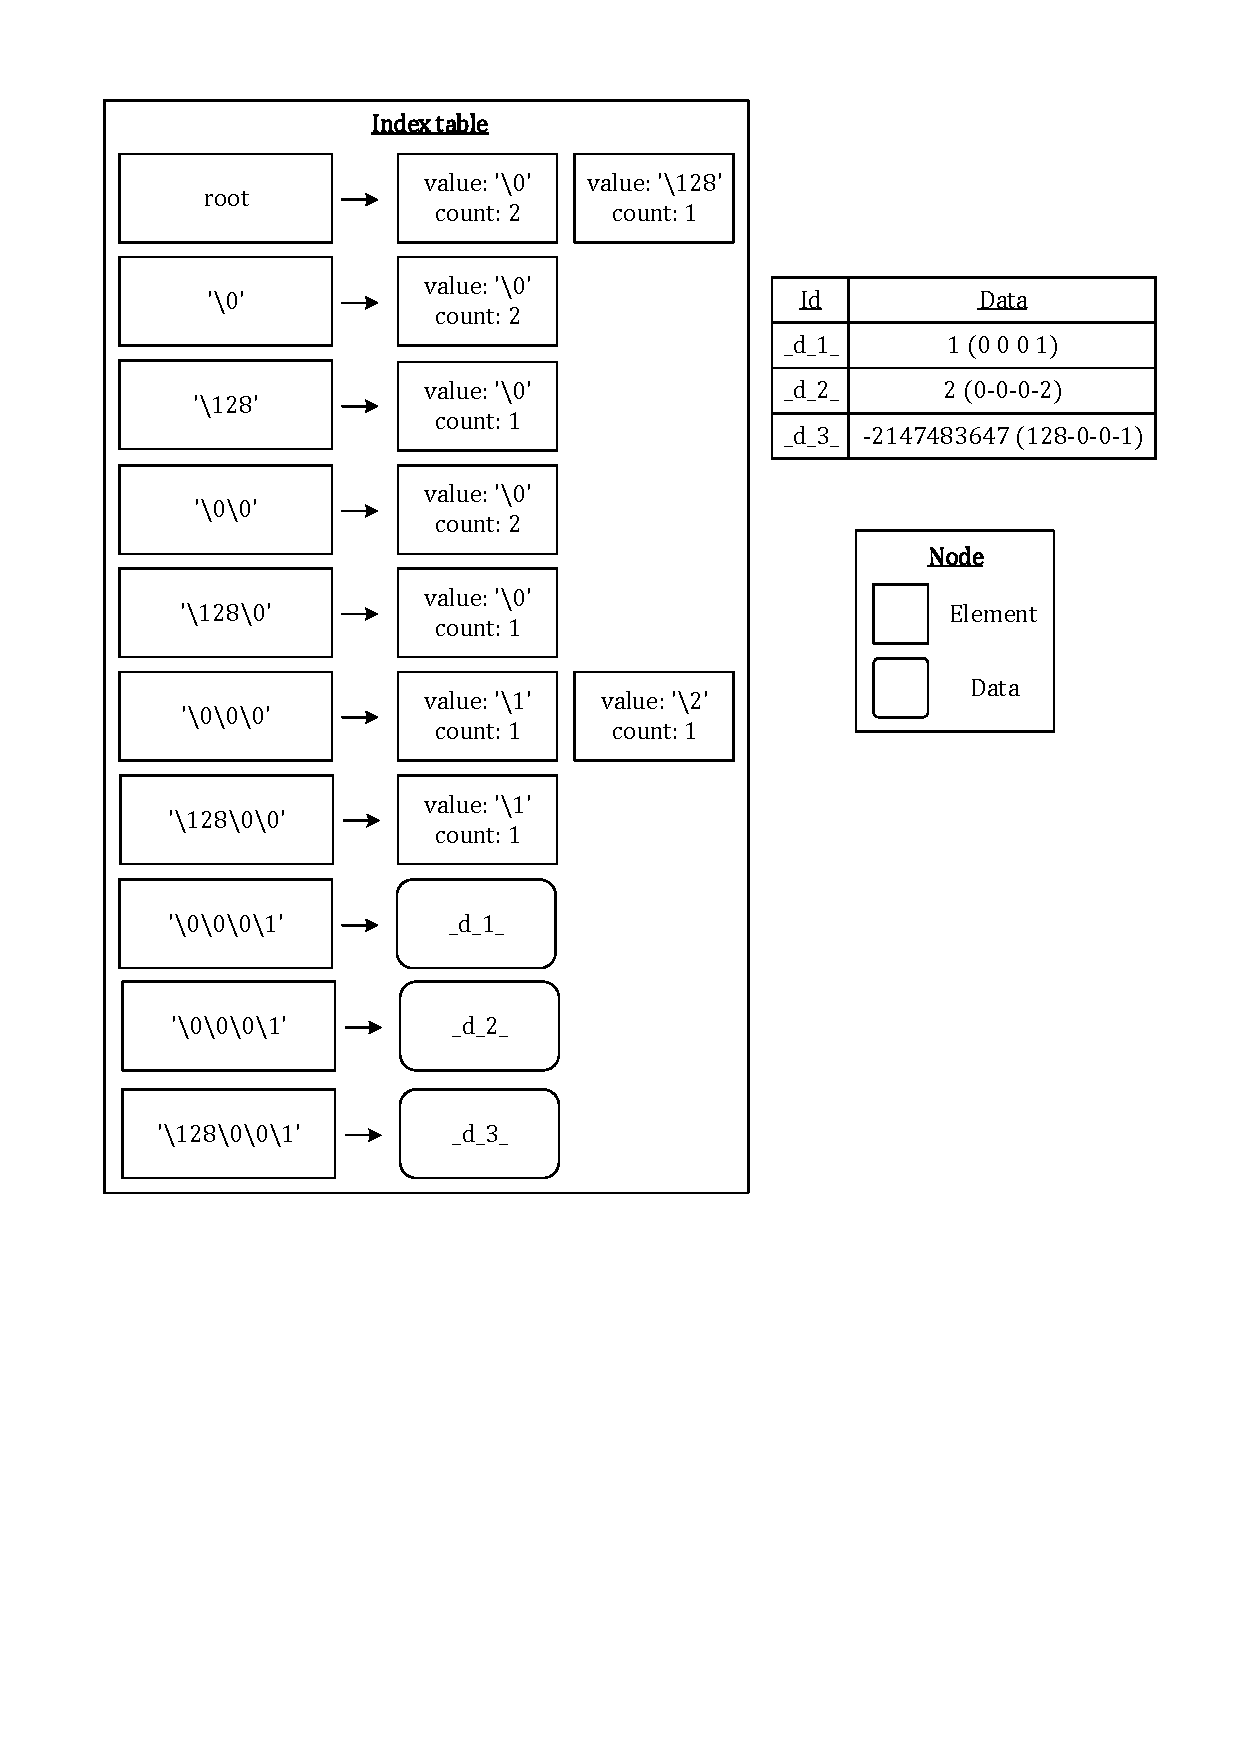
\includegraphics[scale=0.6]{./algorithm/integer/pic/modification/example_1_v3.pdf}
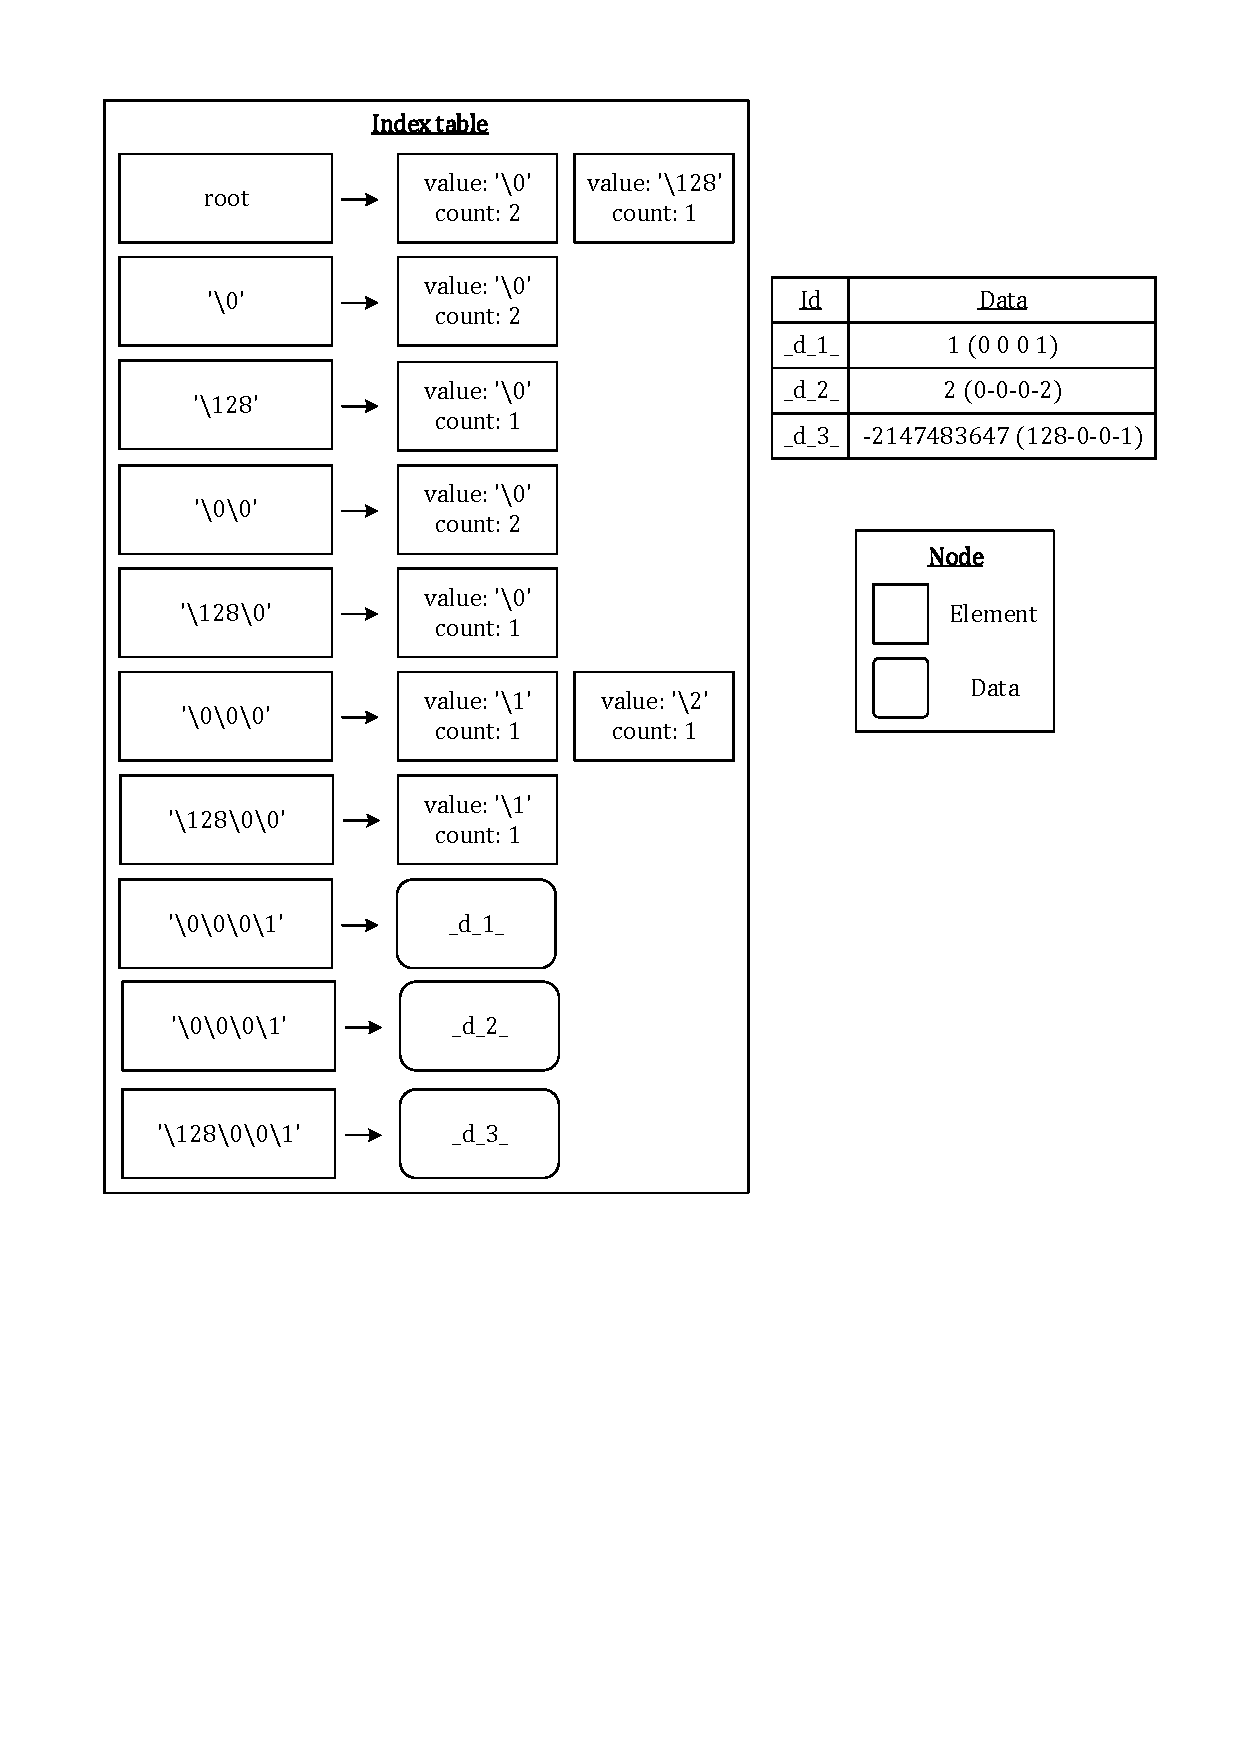
\includegraphics[width=0.8\textwidth]{./algorithm/integer/pic/modification/example_1_v3.pdf}
\caption{The table after modified the value.}
\label{fig:algorithm:integer:modification:example_1}
\end{figure}

